%%%%%%%%%%%%%%%%%%%%%%%%%%%%%%%%%%%%%%%%%
%
% CMPT 424N-111
% Fall 2019
% Lab Five
%
%%%%%%%%%%%%%%%%%%%%%%%%%%%%%%%%%%%%%%%%%

%%%%%%%%%%%%%%%%%%%%%%%%%%%%%%%%%%%%%%%%%
% Short Sectioned Assignment
% LaTeX Template
% Version 1.0 (5/5/12)
%
% This template has been downloaded from: http://www.LaTeXTemplates.com
% Original author: % Frits Wenneker (http://www.howtotex.com)
% License: CC BY-NC-SA 3.0 (http://creativecommons.org/licenses/by-nc-sa/3.0/)
% Modified by Alan G. Labouseur  - alan@labouseur.com
%
%%%%%%%%%%%%%%%%%%%%%%%%%%%%%%%%%%%%%%%%%

%----------------------------------------------------------------------------------------
%	PACKAGES AND OTHER DOCUMENT CONFIGURATIONS
%----------------------------------------------------------------------------------------

\documentclass[letterpaper, 10pt,DIV=13]{scrartcl} 

\usepackage[T1]{fontenc} % Use 8-bit encoding that has 256 glyphs
\usepackage[english]{babel} % English language/hyphenation
\usepackage{amsmath,amsfonts,amsthm,xfrac} % Math packages
\usepackage{sectsty} % Allows customizing section commands
\usepackage{graphicx}
\graphicspath{ {./} }
\usepackage[lined,linesnumbered,commentsnumbered]{algorithm2e}
\usepackage{listings}
\usepackage{parskip}
\usepackage{lastpage}

\allsectionsfont{\normalfont\scshape} % Make all section titles in default font and small caps.

\usepackage{fancyhdr} % Custom headers and footers
\pagestyle{fancyplain} % Makes all pages in the document conform to the custom headers and footers

\fancyhead{} % No page header - if you want one, create it in the same way as the footers below
\fancyfoot[L]{} % Empty left footer
\fancyfoot[C]{} % Empty center footer
\fancyfoot[R]{page \thepage\ of \pageref{LastPage}} % Page numbering for right footer

\renewcommand{\headrulewidth}{0pt} % Remove header underlines
\renewcommand{\footrulewidth}{0pt} % Remove footer underlines
\setlength{\headheight}{13.6pt} % Customize the height of the header

\numberwithin{equation}{section} % Number equations within sections (i.e. 1.1, 1.2, 2.1, 2.2 instead of 1, 2, 3, 4)
\numberwithin{figure}{section} % Number figures within sections (i.e. 1.1, 1.2, 2.1, 2.2 instead of 1, 2, 3, 4)
\numberwithin{table}{section} % Number tables within sections (i.e. 1.1, 1.2, 2.1, 2.2 instead of 1, 2, 3, 4)

\setlength\parindent{0pt} % Removes all indentation from paragraphs.

\binoppenalty=3000
\relpenalty=3000

%----------------------------------------------------------------------------------------
%	TITLE SECTION
%----------------------------------------------------------------------------------------

\newcommand{\horrule}[1]{\rule{\linewidth}{#1}} % Create horizontal rule command with 1 argument of height

\title{	
   \normalfont \normalsize 
   \textsc{CMPT 424N-111 - Fall 2019 - Dr. Labouseur} \\[10pt] % Header stuff.
   \horrule{0.5pt} \\[0.25cm] 	% Top horizontal rule
   \huge Lab Five  \\     	    % Assignment title
   \horrule{0.5pt} \\[0.25cm] 	% Bottom horizontal rule
}

\author{Eric Stenton \\ \normalsize Eric.Stenton1@Marist.edu}

\date{\normalsize\today} 	% Today's date.

\begin{document}
\maketitle % Print the title

%----------------------------------------------------------------------------------------
%   start PROBLEM ONE
%----------------------------------------------------------------------------------------
\section{Problem One}

Consider the following set of processes, with the length of the CPU burst given in milliseconds:

\begin{center}
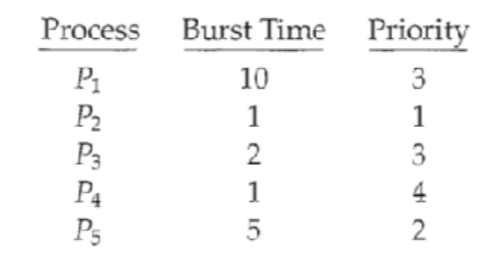
\includegraphics[scale=1.5]{processes}
\end{center}

The processes are assumed to have arrived in the order P1, P2, P3, P4, P5 all at time 0.

a. Draw four Gantt charts that illustrate the execution of these processes using the following scheduling algorithms: FCFS, SJF, nonpreemptive priority (a smaller priority number implies a higher priority), and RR (quantum = 1).

\begin{center}
    FFCS
    
    \begin{tabular}{|c|c|c|c|c|c|c|c|c|c|c|c|c|c|c|c|c|c|c|}
        \hline
        P1 & P1 & P1 & P1 & P1 & P1 & P1 & P1 & P1 & P1 & P2 & P3 & P3 & P4 & P5 & P5 & P5 & P5 & P5 \\    
        0 & 1 & 2 & 3 & 4 & 5 & 6 & 7 & 8 & 9 & 10 & 11 & 12 & 13 & 14 & 15 & 16 & 17 & 18 \\

        \hline
    \end{tabular}
\end{center}

\begin{center}
    SJF
    
    \begin{tabular}{|c|c|c|c|c|c|c|c|c|c|c|c|c|c|c|c|c|c|c|}
        \hline
        P2 & P4 & P3 & P3 & P5 & P5 & P5 & P5 & P5 & P1 & P1 & P1 & P1 & P1 & P1 & P1 & P1 & P1 & P1 \\
        0 & 1 & 2 & 3 & 4 & 5 & 6 & 7 & 8 & 9 & 10 & 11 & 12 & 13 & 14 & 15 & 16 & 17 & 18 \\

        \hline
    \end{tabular}
\end{center}

\begin{center}
    Nonpreemptive Priority
    
    \begin{tabular}{|c|c|c|c|c|c|c|c|c|c|c|c|c|c|c|c|c|c|c|}
        \hline
        P2 & P5 & P5 & P5 & P5 & P5 & P1 & P1 & P1 & P1 & P1 & P1 & P1 & P1 & P1 & P1 & P3 & P3 & P4 \\
        0 & 1 & 2 & 3 & 4 & 5 & 6 & 7 & 8 & 9 & 10 & 11 & 12 & 13 & 14 & 15 & 16 & 17 & 18 \\

        \hline
    \end{tabular}
\end{center}

\begin{center}
    RR (Quantum = 1)
    
    \begin{tabular}{|c|c|c|c|c|c|c|c|c|c|c|c|c|c|c|c|c|c|c|}
        \hline
        P1 & P2 & P3 & P4 & P5 & P1 & P3 & P5 & P1 & P5 & P1 & P5 & P1 & P5 & P1 & P1 & P1 & P1 & P1 \\
        0 & 1 & 2 & 3 & 4 & 5 & 6 & 7 & 8 & 9 & 10 & 11 & 12 & 13 & 14 & 15 & 16 & 17 & 18 \\
        \hline
    \end{tabular}
\end{center}
\vspace{\baselineskip}
b. What is the turnaround time of each process for each of the scheduling algorithms in part a?

FFCS: (10 + 11 + 13 + 14 + 19)/5 = 67/5 = 13.4 

SJF: (19 + 1 + 4 + 2 + 9)/5 = 35/5 = 7 

Non-preepmtive Priority: (16 + 1 + 18 + 19 + 6)/5 = 60/5 = 12

RR (Quantum = 1): (19 + 2 + 7 + 4 + 14)/5 = 46/5 = 9.2 

\vspace{\baselineskip}
c. What is the waiting time of each process for each of these scheduling algorithms?

FFCS: (0 + 10 + 11 + 13 + 14)/5 = 48/5 = 9.6

SJF: (9 + 0 + 2 + 1 + 4)/5 = 16/5 = 3.2 

Non-preepmtive Priority: (6 + 0 + 16 + 18 + 1)/5 = 41/5 =  8.2

RR (Quantum = 1): (9 + 1 + 5 + 3 + 9)/5 = 27/5 = 5.4  

\vspace{\baselineskip}
d. Which of the algorithms results in the minimum average waiting time (over all processes)?

\hspace{20px}The shortest job first (SJF) algorithm results in the minimum average waiting time over all processes which makes sense because it is the optimal, albeit impossible to realistically implement, scheduling algorithm. 

%----------------------------------------------------------------------------------------
%   end PROBLEM ONE
%----------------------------------------------------------------------------------------

%----------------------------------------------------------------------------------------
%   REFERENCES
%----------------------------------------------------------------------------------------
\end{document}
